\documentclass[12pt]{article}
\usepackage{amsmath,latexsym,amsfonts,amssymb,graphicx,amsthm,epsfig,enumerate}
\usepackage{tikz,verbatim,tabularx} % adds charting fuctions
\newcolumntype{C}{>{\centering\arraybackslash}X}
\linespread{1.2}

%\pagestyle{empty}

\begin{document}
	\title{6 Man's Morris: 2AA4/2ME3 Assignment 2} %add title here
	\author{
		Gregory Smilski, 1404091\\
		Abigail Gaulin, 1327924\\
		Karl Knopf 1437217} 
	% add other necessary information here
	
	\maketitle
	\thispagestyle{empty}
	\newpage
	\tableofcontents
	\newpage
	
	\section{Introduction}
	This document describes the java project 6 Men's Morris. 
	\subsection{Architecture}
	\begin{figure}[!h]
		\centering
		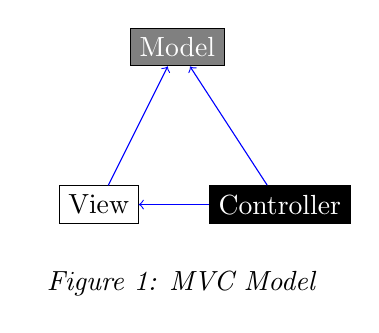
\begin{tikzpicture}
		% MVC Architecture
		\node[draw] (View) at (0,0) {View};
		\node[draw,fill=black,text=white] (Controller) at (2.3,0) {Controller};
		\node[draw,fill=gray,text=white] (Model) at (1,2) {Model};
		
		\draw[->,draw=blue] (View) to (Model);
		\draw[->,draw=blue] (Controller) to (View);
		\draw[->,draw=blue] (Controller) to (Model);
		\node at (1.0, -1.0) {\textit{ Figure 1: MVC Model}};
		
		\end{tikzpicture}
	\end{figure}
	This software uses MVC architecture in its design. MVC stands for Model, View, Controller, and is a design tool used in software development. The View contains all information the user sees, and interacts with the user. The Model contains all the data, and the Controller contains commands which modify the view and model. This architectural style is useful as it allows for modulation, and parts of the program can be modified without affecting any others.
	\subsection{Technologies}
	\begin{itemize}
		\item Java:  An object oriented programming language 
		\item Eclipse: It is an IDE used for the development and testing of software typically in Java
		\item Java Swing: A java toolkit designed to aid programmers in the creation of gui applications. This widget toolkit allows the programmer quick access to various predefined graphical objects, allowing the easy creation of a graphical interface.
		
	\end{itemize}
	\section{Modular Decomposition}
	% 4.1Description of the classes and modules and why they were used
		\begin{figure}[!h]
			\centering
			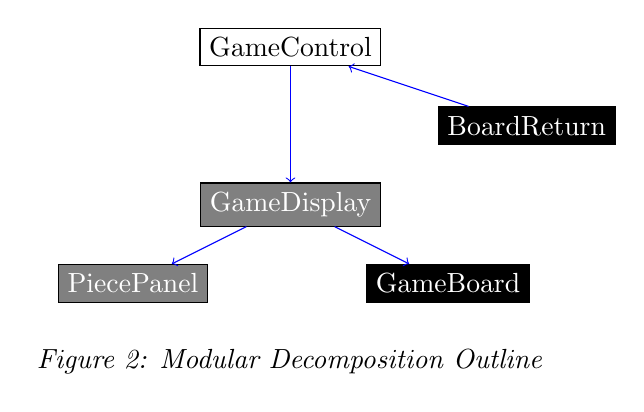
\begin{tikzpicture}
			% MVC Architecture
			\node[draw] (GameControl) at (1,3) {GameControl};
			\node[draw,fill=black,text=white] (GameBoard) at (3,0) {GameBoard};
			\node[draw,fill=gray,text=white] (GameDisplay) at (1,1) {GameDisplay};
			\node[draw,fill=gray,text=white] (PiecePanel) at (-1,0) {PiecePanel};
			\node[draw,fill=black,text=white] (BoardReturn) at (4,2) {BoardReturn};
			
			\draw[->,draw=blue] (GameControl) to (GameDisplay);
			\draw[->,draw=blue] (GameDisplay) to (PiecePanel);
			\draw[->,draw=blue] (GameDisplay) to (GameBoard);
			\draw[->,draw=blue] (BoardReturn) to (GameControl);
			\node at (1.0, -1.0) {\textit{Figure 2: Modular Decomposition Outline}};
			
			\end{tikzpicture}
		\end{figure}
	The modules chosen (as detailed in the Module Guide), were done so in order to make it straightforward for the 3 members involved in the project to code individually, and also to enforce modularity in the program. The GameDisplay, GameBoard and PiecePanel make up the View. The PiecePanel creates the tokens to take the user input, GameDisplay creates buttons to check or restart the game, and GameBoard displays the game data to the user. By dividing the View up in this way, if any of these functionalities need to be modified that can be done without affecting the other parts. The GameControl makes up the Controller. This controls the game logic, and is called by the View to make modifications to the game data based on user input. It makes sense for the Controller to be separate from the other modules, as any changes that are made to the game logic can be implemented without there being any change to what the user sees/interacts with, and likewise any changes to the user interface will not interfere with the game logic/data.
	\newpage
	\section{Module Guide}
	%4.2 For each module, a description of the interface and behaviors of each method
	\subsection{MIS}

	\begin{itemize}
		\item robut.java \\
		This module acts as an Artificial Intelligence to determine what move the computer should make. It is used by GameDisplay.java to give the computer’s next move based on a given board  \\
		\underline{Interface Uses} 
		\begin{itemize}
			\item none
		\end{itemize} 
		\underline{Return Type}
		\begin{itemize}
			\item Information on the game currently being played
		\end{itemize}
		\underline{Access Programs}
		\begin{itemize}
			\item public static int[] place(int[][] visibleTeams, int colour, int added) : A public method that, based on the setup of the board and the number of pieces on it, determines and returns a location on the board where a new piece should be placed.
			\item public static int[] move(int[][] visibleTeams, int colour) : A public method that, based on the setup of the board, determines and returns a set of locations on the board of what piece should be moved and where it should be moved to.
			\item public static int[] mill(int[][] visibleTeams, int colour, int added) : A public method that, based on the setup of the board determines and returns the location of a piece on the board that should be removed.
		\end{itemize}
		\item GameData.java \\
		This module acts as the module in MVC framework, and stores and returns the information for the game currently in play. It is used by GameDisplay.java and Gameboard.java to return and update game data, and by FileIO.java return game data to be saved. \\
		\underline{Interface Uses} 
		\begin{itemize}
			\item FileIO.java
		\end{itemize} 
		\underline{Return Type}
		\begin{itemize}
			\item Information on the game currently being played
		\end{itemize}
		\underline{Access Programs}
		\begin{itemize}
			\item public GameData() : A constructor for GameData class. Allows another class to create Game Data for a new game.
			\item public int[][] getVisibleTeams() : A getter method for the locations of the pieces on the game board.
			\item public void setVisibleTeams(int x, int y, int value) : A setter method for an individual value of visibleTeams. Allows a piece to be added to the gameboard.
			\item public void setVisibleTeams(int[][] newTeams) : A setter method for the whole of visibleTeams. Allows for an old game to be loaded to the game board.
			\item public void incrementPlay1count() : Increments the number of pieces played by player 1 by 1.
			\item public void decreasePlay1count() : Decrements the number of pieces played by player 1 by 1.
			\item public void setPlay1count(int count) : A setter method for the number of pieces played by player 1. Allows for an old game’s count of player 1’s pieces to be loaded.
			\item public int getPlay1count() : A getter method for the number of pieces played by player 1.
			\item public int getPlay1removed() : A getter method for the number of player 1’s pieces that were removed.
			\item public void incrementPlay2count() : Increments the number of pieces played by player 2 by 1.
			\item public void decreasePlay2count() : Decrements the number of pieces played by player 2 by 1.
			\item public void setPlay2count(int count) : A setter method for the number of pieces played by player 2. Allows for an old game’s count of player 2’s pieces to be loaded.
			\item public int getPlay2count() : A getter method for the number of pieces played by player 2.
			\item public int getPlay2removed() : A getter method for the number of player 2’s pieces that were removed.
			\item public void setRedTake(bolean value) : A setter method for whether or not red can take one of blue’s pieces.
			\item public Boolean getRedTake() : A getter method for whether or not red can take one of blue’s pieces.
			\item public void setBlueTake(bolean value) : A setter method for whether or not blue can take one of red’s pieces.
			\item public Boolean getBlueTake() : A getter method for whether or not blue can take one of red’s pieces.
			\item public void incrementTake() : A method that switches which player is active.
			\item public void setFirst(boolean bool) : A setter method that sets which player moves first.
			\item public boolean getFirst() : A getter method that returns which player moves first.
			\item public void setState(int state) : A setter method that sets the previous state to the current state and sets the current state to the new state.
			\item public int getCurrentState() : A getter method that returns the current state of the game.
			\item public int getPreviousState() : A getter method that returns the previous state of the game.
			\item public int getPreviousMoves() : A getter method that returns the number of moves previously made.
			\item public void resetPreviousMoves() : A method that sets the number of previous moves to 0.
			\item public void incrementPreviousMoves() : A method that increases the number of previous moves by 1.
			\item public void loadGame() : A method that loads a game state from a txt file.
		\end{itemize}

	\end{itemize}
		
	\subsection{MID}
	\begin{itemize}
		\item robut.java \\
		\underline{Variables}
		\begin{itemize}
			\item None
		\end{itemize}
		\underline{Access Programs}
		\begin{itemize}
			\item public static int[] place(int[][] visibleTeams, int colour, int added) : A public method taking 3 inputs: visibleTeams, an integer array of the setup of the board; colour, an integer of what which team’s piece is being placed; added, an integer of the number of pieces added to the board. Determines and returns a location on the board where a new piece should be placed.
			\item public static int[] move(int[][] visibleTeams, int colour) : A public method taking 2 inputs: visibleTeams, an integer array of the setup of the board; colour, an integer of what which team’s piece is being placed. Determines and returns a set of locations on the board of what piece should be moved and where it should be moved to.
			\item public static int[] mill(int[][] visibleTeams, int colour, int added) : A public method taking 2 inputs: visibleTeams, an integer array of the setup of the board; colour, an integer of what which team’s piece is being placed. Determines and returns the location of a piece on the board that should be removed.
		\end{itemize}
		\underline{Private Programs}
		\begin{itemize}
			\item private static int[] random(int[][] visibleTeams, int search) : A private method that searches for a random piece of a certain colour on the board and returns its location.
			\item private static in[][] nearMill(int[][] visibleTeams, int colour, int action) : A private method that searches for any near mills of a certain colour and either returns and array of integer arrays of either the empty spots of near mills to be completed or pieces in near mills to be removed.
			\item private static int nearMillRandom(int empty, int pieceA, int pieceB, int action) : A private method that, based on the value of action, either returns the location of the empty spot of a near mill or one of the two pieces in a near mill.
			\item private static int[][] checkAdjacent(int[][] visibleTeams, int adj, int i, int j) : A private method that, given a location and a type to search for (a piece of a certain colour or an empty spot), will return an array of integer arrays of the locations of the adjacent pieces of that type.
			\item private static int[][] checkAdjacent(int[][] visibleTeams, int adj, int i, int j) : A private method that, given a location and a type to search for (a piece of a certain colour or an empty spot), will return an array of integer arrays of the locations of the adjacent pieces of that type.
			\item private static int[][] findMill(int[][] visibleTeams, int notColour) : A private method that searches for any mills that a player has and returns one piece from each mill to be removed.
			\item private static int findMillRandom(int pieceA, int pieceB, int pieceC) : A private method that, given a mill, randomly returns one of the three pieces to be removed.
			\item private static int[] nearbyPiece(int[][] visibleTeams, int[][] nearMills, int search) : A private method that, given an array of locations of near mills, will search for and return the location of a nearby piece of a certain colour to block or complete the near mill, if one exists.
		\end{itemize}
		\item GameData.java \\
		\underline{Variables}
		\begin{itemize}
			\item private int[][] visibleTeams : An integer array of the current state of each piece.
			\item private boolean redTake : A boolean to mark whether or not red is the active player. If true, red is active. If not, red is not active.
			\item private boolean blueTake : A boolean to mark whether or not blue is the active player. If true, blue is active. If not, blue is not active.
			\item private boolean first : A boolean that represents which player goes first.
			\item private int currentState : An integer to mark which state the game is currently in.
			\item private int previousState : An integer to mark which state the game was in before it became its current state.
			\item private int play1count : The number of active pieces for player 1.
			\item private int play2count : The number of active pieces for player 2.
			\item private int play1removed : The number of pieces of player 1’s that have been removed.
			\item private int play2removed : The number of pieces of player 2’s that have been removed.
			\item private int previousMoves : The number of moves that have been made in the game.
			\item private final int allowable : The maximum number of pieces each player is allowed to have.
			
		\end{itemize}
		\underline{Access Programs}
		\begin{itemize}
			\item public GameData() : A constructor for GameData class. Allows another class to create Game Data for a new game.
			\item public int[][] getVisibleTeams() : A getter method for the locations of the pieces on the game board.
			\item public void setVisibleTeams(int x, int y, int value) : A setter method for an individual value of visibleTeams. Allows a piece to be added to the gameboard.
			\item public void setVisibleTeams(int[][] newTeams) : A setter method for the whole of visibleTeams. Allows for an old game to be loaded to the game board.
			\item public void incrementPlay1count() : Increments the number of pieces played by player 1 by 1.
			\item public void decreasePlay1count() : Decrements the number of pieces played by player 1 by 1.
			\item public void setPlay1count(int count) : A setter method for the number of pieces played by player 1. Allows for an old game’s count of player 1’s pieces to be loaded.
			\item public int getPlay1count() : A getter method for the number of pieces played by player 1.
			\item public int getPlay1removed() : A getter method for the number of player 1’s pieces that were removed.
			\item public void incrementPlay2count() : Increments the number of pieces played by player 2 by 1.
			\item public void decreasePlay2count() : Decrements the number of pieces played by player 2 by 1.
			\item public void setPlay2count(int count) : A setter method for the number of pieces played by player 2. Allows for an old game’s count of player 2’s pieces to be loaded.
			\item public int getPlay2count() : A getter method for the number of pieces played by player 2.
			\item public int getPlay2removed() : A getter method for the number of player 2’s pieces that were removed.
			\item public void setRedTake(bolean value) : A setter method for whether or not red can take one of blue’s pieces.
			\item public Boolean getRedTake() : A getter method for whether or not red can take one of blue’s pieces.
			\item public void setBlueTake(bolean value) : A setter method for whether or not blue can take one of red’s pieces.
			\item public Boolean getBlueTake() : A getter method for whether or not blue can take one of red’s pieces.
			\item public void incrementTake() : A method that switches which player is active.
			\item public void setFirst(boolean bool) : A setter method that sets which player moves first.
			\item public boolean getFirst() : A getter method that returns which player moves first.
			\item public void setState(int state) : A setter method that sets the previous state to the current state and sets the current state to the new state.
			\item public int getCurrentState() : A getter method that returns the current state of the game.
			\item public int getPreviousState() : A getter method that returns the previous state of the game.
			\item public int getPreviousMoves() : A getter method that returns the number of moves previously made.
			\item public void resetPreviousMoves() : A method that sets the number of previous moves to 0.
			\item public void incrementPreviousMoves() : A method that increases the number of previous moves by 1.
			\item public void loadGame() : A method that loads a game state from a txt file.
			
		\end{itemize}
		\underline{Private Programs}
		\begin{itemize}
			\item None
		\end{itemize}
		
		
	
	
	\end{itemize}
	\section{Traceability}
	% 4.5 A Description of each class
	% Tablular Expressions
	\begin{tabularx}{\linewidth}{|C|C|C|}
		\hline \\
		Requirement & Module & Result \\
		\hline
		Random Player selected to go First & GameControl & random boolean generated to represent either player 1 or player 2 \\
		\hline \\
		Setting up Board Array & GameControl & int[][] generated to hold values at each position on array. Initially, the array holds all zeros, representing no disks on board. \\
		\hline \\
		Checking if New Piece Position is Legal & GameControl & If the position is legal (no other pieces already in that position), returns a 1 and the new array, otherwise returns a 0 and the old array. \\ 
		\hline \\
		Checking if Moved Piece Position is Legal & GameControl & If the position is legal (no other pieces in that position, it is an adjacent position), returns a 1 and the new array, otherwise returns a 0 and the old array.\\
		\hline \\
		Displaying an array as a Six Men's Morris Board &
		GameBoard & Game is Displayed as a panel on a jFrame, allows for user interaction \\ 
		\hline \\
		Allowing the user to place a piece & GameBoard &
		User is able to select a location and place a piece \\
		\hline \\
	\end{tabularx}
		\begin{tabularx}{\linewidth}{|C|C|C|}
			\hline \\
			Requirement & Module & Result \\
			\hline \\
			The pieces used in the game are red and blue & GameBoard & The gameboard draws the pieces and restricts their colors to red and blue \\
			\hline \\
			Requirement & Module & Result \\
			\hline \\
			Starting with an empty board displayed & GameBoard & All of the spaces are initial empty (black) on the gameboard. \\
			\hline \\
			New Game Button & GameDisplay & Allows user to select option to restart the board, will call GameControl. \\
			\hline \\
			Check Button & GameDisplay  & Allows user to check if current board is legal, will call GameControl. \\
			\hline \\
			User-Game Interaction & GameDisplay &Allows user to interact with game pieces, make modifications to current board, will call GameControl. \\
			\hline \\	
	\end{tabularx}
		\begin{tabularx}{\linewidth}{|C|C|C|}
			\hline \\
			Requirement & Module & Result \\
			\hline \\
			Game is able to recognize a Winner & Game Display & Game has criteria to meet (player only has 2 pieces left) to determine if there is a winner \\
			\hline \\
			Players are only able to make legal moves & BoardReturn & Game is able to determine which moves are legal and only allows player to make correct moves \\
			\hline \\
			Players make moves in turn & Game Display & Game alternates player turns, and displays the current player to the screen \\
			\hline \\
			Users can save a game & Game Display & Users can use a button to save their current game to a text file \\
			\hline \\
			Users can load a game & Game Display & Users can use a button to load their current game from a text file \\
			\hline
				
		\end{tabularx}
	
	\section{Uses Relation}
	% A diagram and brief description describing why how the stuff interacts
			\begin{figure}[!h]
				\centering
				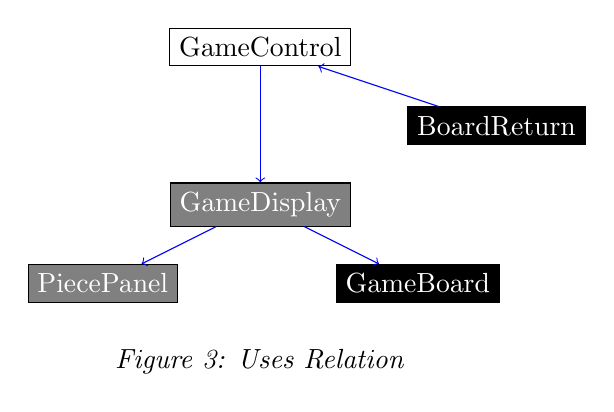
\begin{tikzpicture}
			\node[draw] (GameControl) at (1,3) {GameControl};
			\node[draw,fill=black,text=white] (GameBoard) at (3,0) {GameBoard};
			\node[draw,fill=gray,text=white] (GameDisplay) at (1,1) {GameDisplay};
			\node[draw,fill=gray,text=white] (PiecePanel) at (-1,0) {PiecePanel};
			\node[draw,fill=black,text=white] (BoardReturn) at (4,2) {BoardReturn};
			
			\draw[->,draw=blue] (GameControl) to (GameDisplay);
			\draw[->,draw=blue] (GameDisplay) to (PiecePanel);
			\draw[->,draw=blue] (GameDisplay) to (GameBoard);
			\draw[->,draw=blue] (BoardReturn) to (GameControl);
				\node at (1.0, -1.0) {\textit{Figure 3: Uses Relation}};
				
				\end{tikzpicture}
			\end{figure}
	In the above relation, a class points to another that it uses.
	The View calls the Controller, which in turn modifies the Model. In the future, the View will initially take input from the user. Then, depending on which component was clicked, will call a corresponding method in the controller. Clicking either the red or blue piece will call the newpiece method in GameControl. Clicking the check button will call checkboard(), and clicking the start button will call startboard(). These methods will then modify the model through the manipulation of arrays. \\
	\newpage
	\section{Computer Player AI}	
	\indent The computer player was designed with the three states of gameplay in mind. Just as the player was implemented through parsing inputs in differing methods depending on the state of the game, the computer was implemented as an abstract class that returns inputs of where to move next depending on which state the game is in. For each state there is a corresponding function to determine what move the computer player should make: place() corresponds with state 1; move() corresponds with state 2; mill() corresponds with state 3.\\
	The computer player was designed with the three states of gameplay in mind. Just as the player was implemented through parsing inputs in differing methods depending on the state of the game, the computer was implemented as an abstract class that returns inputs of where to move next depending on which state the game is in. For each state there is a corresponding function to determine what move the computer player should make: place() corresponds with state 1; move() corresponds with state 2; mill() corresponds with state 3.\\
	The function move() works in a similar fashion. It begins by checking if the computer has a near mill. If it has that it continues to check for whether there is one of the computer’s pieces adjacent to the empty spot of the near mill. If that is true, then the piece is moved to complete the mill. However, if any one of those are false move() checks if the other player has a near mill. If true, it continues to check for whether one of the computer’s pieces is adjacent to the empty spot of the opponent’s near mill. If that is also true, the piece is moved to block the other player from creating a mill. If all else fails, a random piece of the computer’s is moved to a random open adjacent location.\\
	Finally, mill()’s implementation follows that of move() and place(). It begins by checking if the opposing player has a mill and, if it does, randomly removes one of the three pieces that make up the mill. If the opponent does not have a mill, the function checks if they have a near mill instead and removes one of the pieces that makes it up, if it exists. Otherwise, mill() randomly removes one of the opponent’s pieces.\\
	\section{Testing}
	% A section on the testing of the software
	%Behavoir Table
	
	\begin{tabularx}{\linewidth}{|C|C|C|}
		\hline
		What was Tested & What it did & Comments \\
		\hline \\
    GameControl: startboard & Printed out 'visibleteams' array & startboard is correctly setting up the 'visibleteams' array \\
    \hline \\
    GameControl: startboard & Printed out "first" boolean & "first" is correctly assigned random boolean values (on 3 separate tests was assigned true, false, and false) \\
    \hline \\
    GameControl: newpiece & Entered various input values (ie: 1,1,true) & Values were correctly entered into 'visibleteams' (ie: visibleteams[1][1] = 1) \\
    \hline \\
    GameControl: newpiece & Was unable to place new peices in spots already occupied (ie: visibleteams[1][1] = 1, then a newpeice was entered there) & An int value of 0 was returned (meaning the move was not legal) and the array was unchanged. \\ 
    \hline \\
    GameControl: movepiece & Ran function while no illegal moves attempted & Correctly returned no errors, updated array correctly \\
    \hline \\
    GameControl: movepiece & Attempted to move pieces illegally on top of each other (ie: piece at [0][0] moved ontop of another piece at [0][1]) & Returned 0, no changes made to 'visibleteams' array (piece remained at [0][0], no other pieces were moved) \\
    \hline \\
	\end{tabularx}
	
	\begin{tabularx}{\linewidth}{|C|C|C|}
		\hline
		What was Tested & What it did & Comments \\
		\hline \\
		 GameControl: movepiece & Attempted to move pieces illegally to positions not adjacent to the current position & Returned 0, no changes made to 'visibleteams' array (piece remained at [0][0]) \\    
		 \hline \\
		GameBoard: GameBoard() & Display the board, allow for color change of disks & Constructor Method for the gameboard panel. Displays the board as a set of pieces. \\
		\hline
		GameBoard: GameBoard() Change Piece Color& Pieces Change color & The display was successfully able to read in the current color array. \\
		\hline
	
		GameDisplay: GameDisplay() & Displayed panel in correct position in frame with buttons in correct positions in panel & GameDisplay is correctly setting up the panel \\
		\hline
		GameDisplay: GameDisplay()& Clicked on "New Game?" Button,  printed "New Game!" in command line & GameDisplay is correctly running through correct output for the given input \\
		\hline
		GameDisplay: GameDisplay() & Clicked on "Check!" Button, printed "Is is correct?" in command line & GameDisplay is correctly running through corect output for the given input \\
		\hline
		PiecePanel: PiecePanel() & Displayed panel in correct position in frame with circle tokens in correct position in panel & PiecePanel is correctly setting up the panel \\
		\hline
	\end{tabularx}
	\newpage
	\begin{tabularx}{\linewidth}{|C|C|C|}
		\hline
		What was Tested & What it did & Comments \\
		\hline 
		PiecePanel: PiecePanel() & Clicked on Red Circle, Displayed "add red?" & PiecePanel is giving the correct output for the given input and is ready to add a red piece to the board \\
		\hline
		PiecePanel: PiecePanel() &  Clicked on Blue Circle, Displayed "add blue?" & PiecePanel is giving the corect output for the given input and is ready to add a blue piece to the board \\
		\hline
		PiecePanel: PiecePanel()  , Clicked on Red Circle, then white circle & White Cirtcle turned red & PiecePanel is giving the corect output for the given input and should add a red piece to the board \\
		\hline
		PiecePanel: PiecePanel()  , Clicked on Red Circle, then white circle that has been coloured red & No output occurred & PiecePanel is giving the corect output for the given input and any additional red peices were not added not on their turn \\
		\hline
		PiecePanel: PiecePanel()  , Clicked on Blue Circle, then white circle that has been coloured red & The red coloured white circle turned blue & PiecePanel is giving the corect output for the given input and a blue piece should be added \\
		\hline
		PiecePanel: PiecePanel()  , Clicked on Blue Circle, then white circle & White Circle turned Blue & PiecePanel is giving the corect output for the given input and should add a blue piece to the board \\
		\hline
		PiecePanel: PiecePanel()  , Clicked on Blue Circle, then white circle that has been coloured blue & No output occurred & PiecePanel is giving the corect output for the given input and any additional red peices were not added not on their turn \\
		\hline
	\end{tabularx}
	\newpage
	\begin{tabularx}{\linewidth}{|C|C|C|}
		\hline
		What was Tested & What it did & Comments \\
		\hline 
		PiecePanel: PiecePanel()  , Clicked on Red Circle, then white circle that has been coloured blue & The blue coloured white circle turned red & PiecePanel is giving the corect output for the given input and a red piece should be added \\
		\hline
		GameDisplay & Attempted to add pieces to board & Pieces were added correctly. Game state (adding pieces) was displayed until each player had 6 pieces on board, turn system working correctly, and current turn was displayed. It was not possible to add pieces on top of each other. \\
		\hline
		GameDisplay & Attempted to move pieces across board & Pieces were only able to move to legal positions (adjacent), no flying was possible. Which players turn it was and when a piece was selected were displayed. \\
		\hline
		GameDisplay & Attempted to mill & When pieces were milled, state was displayed. Successfully deleted other players piece when mill formed. Game continued to function thereafter.\\ 
		\hline
		\end{tabularx}
		\newpage
		\begin{tabularx}{\linewidth}{|C|C|C|}
		\hline
		What was Tested & What it did & Comments \\
		\hline
		GameDisplay & Attempted to win game & When player is down to 2 pieces, the other player's winning status is displayed. \\
		\hline
		GameDisplay & Attempted to save and load game & Game saved and reloaded correctly, all pieces where they were left. \\  
		\hline
	\end{tabularx}
	\section{Discussion}
	%4.6 Internal review/ evaluation of design
	The design follows the MVC format very roughly. As it currently stands, the Model, View, and Controller are all spread across the same few classes: the Model is implemented in GameControl; the View is implemented in GameBoard, PiecePanel, and GameDisplay; and the Controller is implemented in GameDisplay. Each class, particularly GameDisplay, is doing much more than it should. Future iterations will have more modularized code, with features such as saving and loading being within their own class. If asked to judge the program, the group would give it a 7.5/10.
	\subsection{Anticipated Changes}
	% what was designed in anticipation of changes
	\begin{itemize}
	\item    GameControl: Will be able to track previous movements of pieces in the 'visibleteams' array (at present, can only add new pieces in and move them around). Arrays were designed to contain variables that could be modified in the future to reflect these changes. This could be used to implement the behavior of the AI in future projects. 
	In the future, the GameControl could be easily used with different dimensions (ie: 8 Men's Morris).  
	\item    Boardreturn: Class designed to hold variables needed to determine whether a move/new piece is legal. Returns a integer indicating the legality, and a int[][], indicating the current board array. Due to the design of a separate type to bundle this data, if any other data feedback is required in the future, it will be simple to add it in.
	\end{itemize}
	
\end{document}